
        
{It is safe to assume that we can consider the density found out by using the \textbf{vernier caliper} method as the actual density because this is the method that produced the lowest amount of uncertainity relative to other methods.}

{If we are to compare our findings with the desities of known metals, we would come to the conclusion that, the \textbf{given metal block is made up of iron}.}

{$\therefore \text{percentage uncertanity in measurement by ruler} = \left(1 - \frac{\rho_{c2}}{\rho_{c1}}\right)\cdot 100 \approx 16 \%$}

{$\text{percentage uncertanity in measurement by archimedes principle} = \left(1 - \frac{\rho_{c3}}{\rho_{c1}}\right)\cdot 100 \approx 15 \%$}

\begin{figure}[H]
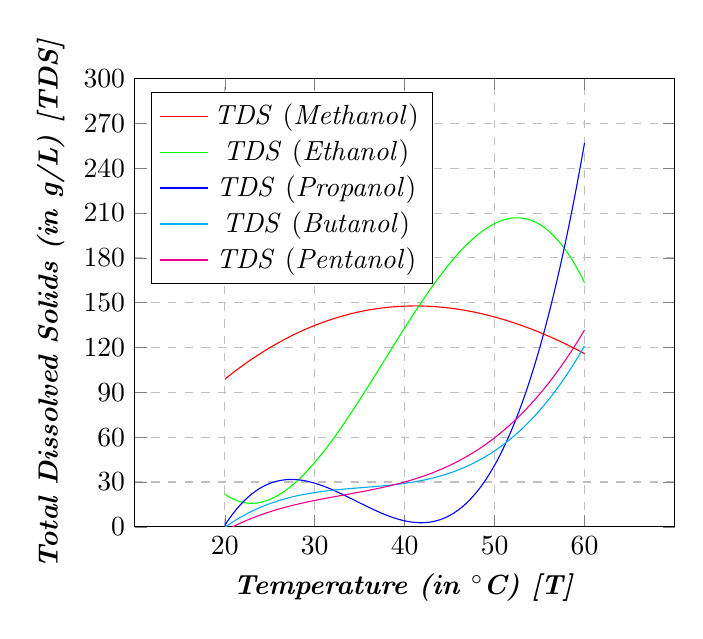
\begin{tikzpicture}
            \begin{axis}[
%                title={\textit{Graph in relation to the \textbf{experimental} \& \textbf{simulation} values of \textbf{drag force} versus \textbf{temperature}}},
                xlabel={\textbf{\textit{Temperature (in $\bm{^\circ}$C) [T]}}},
                ylabel={\textbf{\textit{Total Dissolved Solids (in g/L) [TDS]}}},
                xmin=10, xmax=70,
                ymin=0, ymax=300,
                xtick={20,30,40,50,60},
                ytick={0,30,60,90,120,150,180,210,240,270,300},
                legend pos=north west,
                ymajorgrids=true,
                xmajorgrids=true,
                grid style=dashed,
                legend entries={\textit{TDS} (\textit{Methanol}), \textit{TDS} (\textit{Ethanol}), \textit{TDS} (\textit{Propanol}), \textit{TDS} (\textit{Butanol}), \textit{TDS} (\textit{Pentanol})}
            ]

%			Methanol
            
			\addplot [
    	domain=20:60, 
    	samples=1000, 
    	color=red,
			]
	{(0.000483)*x^3 + (-0.1588)*x^2 + (10.62)*x + (-53.92)};

%			Ethanol

			\addplot [
    	domain=20:60, 
    	samples=1000, 
    	color=green,
			]
	{(-0.01486)*x^3 + (1.682)*x^2 + (-53.754)*x + (543.16)};

%			Propanol

			\addplot [
    	domain=20:60, 
    	samples=1000, 
    	color=blue,
			]
	{(0.01932)*x^3 + (-2.006)*x^2 + (66.4161)*x + (-679.48)};

%			Butanol

			\addplot [
    	domain=20:60, 
    	samples=1000, 
    	color=cyan,
			]
	{(0.005467)*x^3 + (-0.5778)*x^2 + (20.8319)*x + (-229.56)};

%			Pentanol

			\addplot [
    	domain=20:60, 
    	samples=1000, 
    	color=magenta,
			]
	{(0.004216)*x^3 + (-0.4197)*x^2 + (15.0155)*x + (-168.88)};
               
            \end{axis}
%            \caption{\textit{Graph in relation to the \textbf{experimental} \& \textbf{simulation} values of \textbf{drag force} versus \textbf{temperature}}}
        \end{tikzpicture}
        \caption{\textit{Graph in relation to the \textbf{regression line} of \textbf{TDS} versus \textbf{temperature}}}}
		\end{figure}

